\documentclass[final]{beamer}
\def\RightLogoWidth{0.7}
\def\RightLogo{/Users/willbarnes/Documents/Rice/Posters/RiceLogo_TMCMYK300DPI.jpg}
\def\LeftLogoWidth{1.3}
\def\LeftLogo{/Users/willbarnes/Documents/Rice/Posters/coronal_loops_workshop_VII_logo.jpg}
\mode<presentation>
{
\usetheme{I6dv}
}
\setbeamertemplate{caption}[numbered]
%Include packages
\usepackage{soul,color,verbatim}
\usepackage{type1cm}
\usepackage{calc} 
\usepackage{times,mathptmx}
\usepackage{amsmath,amsthm, amssymb, latexsym}
\usepackage{empheq}
\usepackage{graphicx}
\usepackage{epstopdf}
\usepackage[numbers]{natbib}
\usepackage{multicol}
\usepackage{subfigure}
\usepackage[english]{babel}
\usepackage[latin1]{inputenc}
\usepackage[orientation=portrait,size=a0,scale=1.0,debug]{beamerposter}
%Define new commands here
\newcommand{\ang}{\AA~}
\newcommand*\widefbox[1]{\fbox{\hspace{2em}#1\hspace{2em}}}
\newcommand{\figwidth}{0.49}
\setbeamerfont{caption}{size=\footnotesize}

%Set author and title
\title[Two-fluid Effects and EM]{Efficient Modeling of Two-fluid Coronal Plasma:\\Effects of Electron and Ion Heating on Emission Measure}
\author[Barnes \& Bradshaw]{Will T. Barnes \& Stephen J. Bradshaw}
\institute[Rice University]{Department of Physics and Astronomy, Rice University}
\date{21-23 July, 2015}

%Start poster
\begin{document}
\begin{frame}
	\begin{columns}[t]
		\hfill
		%first column
		\begin{column}{0.49\linewidth}
			%Introduction
			\begin{block}{Introduction}
				\begin{itemize}
					\item Nanoflare model of \citet{parker_nanoflares_1988} characterized by energy release on short timescales (e.g. $<200$ s)
					\item Single-fluid models tacitly assume electron and ion populations in equilibrium $\rightarrow$ violated if heating time scale is less than the equilibration (collisional) timescale between the two species
					\item Two-fluid models often assume that electrons are heated, though ion heating mechanisms have been proposed \citep[see][]{markovskii_intermittent_2004}
					\item Hydrodynamic simulations and forward-modeling allow for calculations of observables that provide signatures of different heating mechanisms
					\item We have adapted the enthalpy-based thermal evolution of loops (EBTEL) model of \citet{klimchuk_highly_2008,cargill_enthalpy-based_2012,cargill_enthalpy-based_2012-1} to calculate the \alert{temperature and pressure evolution of the electron and ion populations separately} while assuming quasi-neutrality (i.e. $n_e=n_i=n$)
					\item \textbf{Goal:} Identify differing observational signatures of \alert{electron-versus-ion heating for varying heating frequency} through efficient hydrodynamic simulations
				\end{itemize}
			\end{block}
			%Equations
			\begin{block}{Two-fluid EBTEL Model}
				\begin{itemize}
					\setlength\itemsep{1em}
					%\item The field-aligned two-fluid hydrodynamic equations are,
					%\begin{align}
						%\frac{\partial\rho}{\partial t} &= -\frac{\partial(\rho v)}{\partial s} \label{eq:1dmass} \\[0.5em]
						%\frac{\partial(\rho v)}{\partial t} &= -\frac{\partial(\rho v^2)}{\partial s}-\frac{\partial(p_e + p_i)}{\partial s} + \frac{\partial}{\partial s}\left(\frac{4}{3}\mu_i\frac{\partial v}{\partial s}\right) + \rho g_{\parallel} \label{eq:1dmom} \\[0.5em]
						%\frac{\partial E_e}{\partial t} &= -\frac{\partial}{\partial s} \lbrack(E_e+p_e)v\rbrack+v\frac{\partial p_e}{\partial s} - \frac{\partial F_{c,e}}{\partial s} + \frac{1}{\gamma - 1}k_Bn\nu_{ei}(T_i-T_e) -E_R+E_{H,e} , \label{eq:1denergy_e} \\[0.5em]
						%\frac{\partial E_i}{\partial t} &= -\frac{\partial }{\partial s}\lbrack(E_i+p_i)v\rbrack-v\frac{\partial p_e}{\partial s} - \frac{\partial F_{c,i}}{\partial s} + \frac{1}{\gamma - 1}k_Bn\nu_{ei}(T_e-T_i) + \frac{\partial}{\partial s}\left(\frac{4}{3}\mu_iv\frac{\partial v}{\partial s}\right) +\rho v g_{\parallel} + E_{H,i}.\label{eq:1denergy_i}
					%\end{align}
					%\item Subject to the closure conditions:
					%\begin{enumerate}
					%	\setlength\itemsep{0.5em}
					%	\item $E_e = 1/(\gamma - 1)P_e,~E_i = 1/(\gamma - 1)P_i + 1/2\rho v^2$
					%	\item $p_e=k_BnT_e,~p_i=k_BnT_i$
					%\end{enumerate}
					\item Make the following assumptions as outlined in \citet{klimchuk_highly_2008,cargill_enthalpy-based_2012}:
					\begin{enumerate}
						\setlength\itemsep{0.5em}
						\item Bulk flow is subsonic $\rightarrow$ neglect terms $\mathcal{O}(v^2)$
						\item Loop is shorter than a gravitational scale height ($z<H_g$) $\rightarrow$ neglect gravitational terms
						\item Transition region length $\ell\ll L$,  the coronal loop half-length $\rightarrow$ neglect terms $\mathcal{O}(\ell)$
						\item Semi-circular loop symmetric about the apex
						\item $c_2=\bar{T}/T_a$ and $c_3=T_0/T_a$ are constant and independent of species.
						\item Equations closed by ideal gas law for both species $\rightarrow$ $p_e=k_BnT_e,~p_i=k_BnT_i$
					\end{enumerate} 
					\item Applying these assumptions to the field-aligned two-fluid hydrodynamic equations and integrating over the coronal and transition region portions of the loop, we derive \alert{two-fluid, time-dependent, spatially-averaged equations for $n,~T_e,~T_i,~p_e,~p_i$},
					\begin{empheq}[box=\widefbox]{align}
						\frac{d}{dt}\bar{n} &= \frac{c_2(\gamma-1)}{c_3\gamma Lk_B\bar{T}_e}(\psi_{TR} - F^{(0)}_{c,e}-\mathcal{R}_{TR}),\label{eq:ebtf_n} \\[0.5em]
						\frac{d}{dt}\bar{p}_e &= \frac{\gamma - 1}{L}[\psi_{TR} + \psi_C -(\mathcal{R}_{TR} + \mathcal{R}_C)] + k_B\bar{n}\nu_{ei}(\bar{T}_i-\bar{T}_e) + (\gamma-1)\bar{E}_{H,e},\label{eq:ebtf_pe} \\[0.5em]
						\frac{d}{dt}\bar{p}_i &= -\frac{\gamma - 1}{L}(\psi_{TR} + \psi_C) + k_B\bar{n}\nu_{ei}(\bar{T}_e-\bar{T}_i) + (\gamma-1)\bar{E}_{H,i},\label{eq:ebtf_pi} \\[0.5em]
						\frac{d\bar{T}_{e,i}}{dt} &= \bar{T}_{e,i}\left(\frac{1}{\bar{P}_{e,i}}\frac{d\bar{P}_{e,i}}{dt} - \frac{1}{\bar{n}}\frac{d\bar{n}}{dt}\right),\label{eq:ebtf_tei}
					\end{empheq}
					where
					\begin{align*}
						\psi_{TR} =  \int_{TR}\mathrm{d}s~v\frac{d}{ds}p_e \approx \frac{1}{1 + \xi}(F^{(0)}_{c,e} + \mathcal{R}_{TR} - \xi F^{(0)}_{c,i}),\quad
						\psi_{C} = \int_{C}\mathrm{d}s~v\frac{d}{ds}p_e \approx \bar{v}p_e^{(a)} - (p_ev)_0,\quad
						\xi = \frac{T_e^{(0)}}{T_i^{(0)}}.
					\end{align*} 
				\end{itemize}
			\end{block}
			%Comparison
			\begin{block}{Benchmarking with 1D Hydrodynamic Models}
				\begin{itemize}
					\item Field-aligned hydrodynamic code HYDRAD \citep{reep_diagnosing_2013} used to benchmark two-fluid EBTEL model
					\item 0D models such as EBTEL allow for large parameter-space explorations while also capturing (most of) the complex physics of dynamic coronal loops
					\item Good agreement with 1D model despite HYDRAD incorporating a lot more physics (e.g. shocks, flows, non-equilibrium ionization)
				\end{itemize}
				\begin{figure}[htp]
					\centering
					\subfigure[]{%
					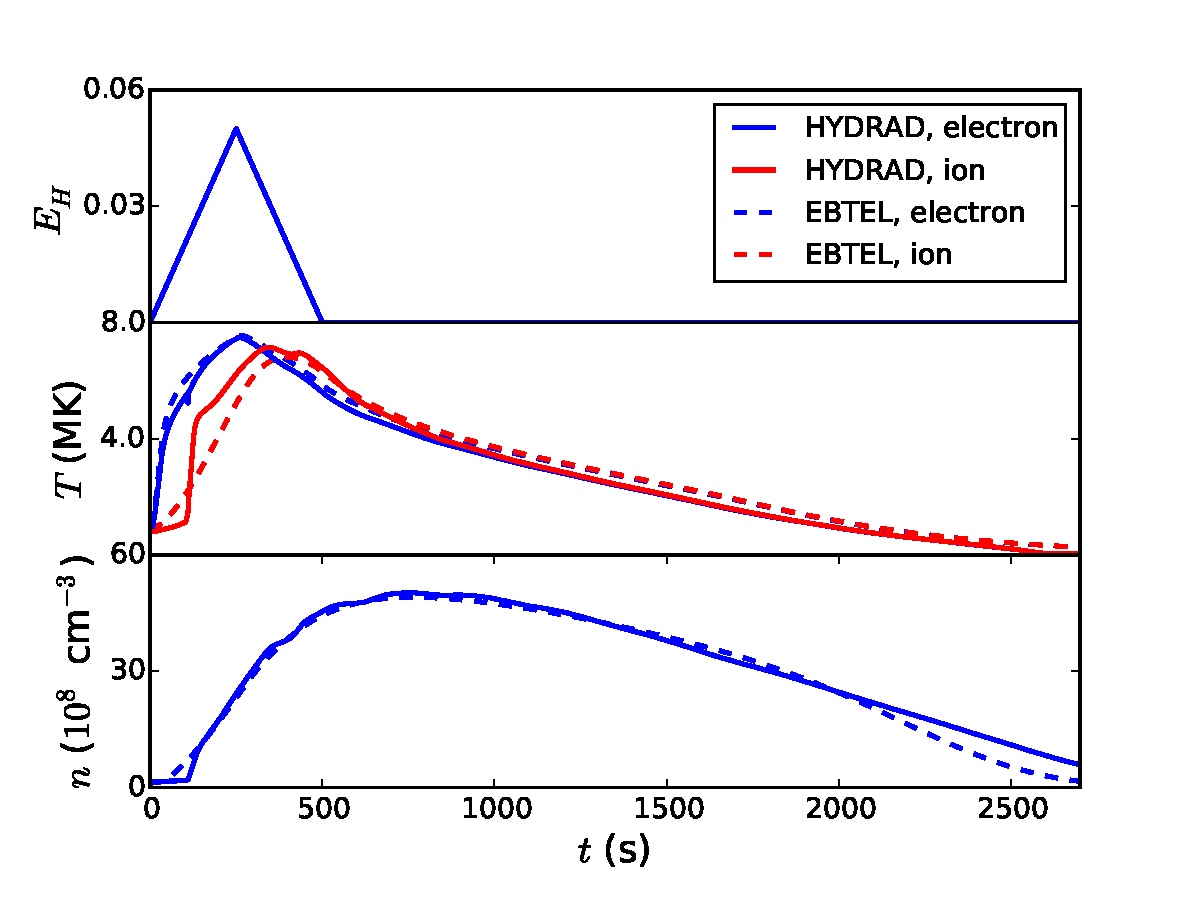
\includegraphics[width=\figwidth\columnwidth]{figures/compare_1_event.pdf}
					\label{fig:compare_1_event}}
					\subfigure[]{%
					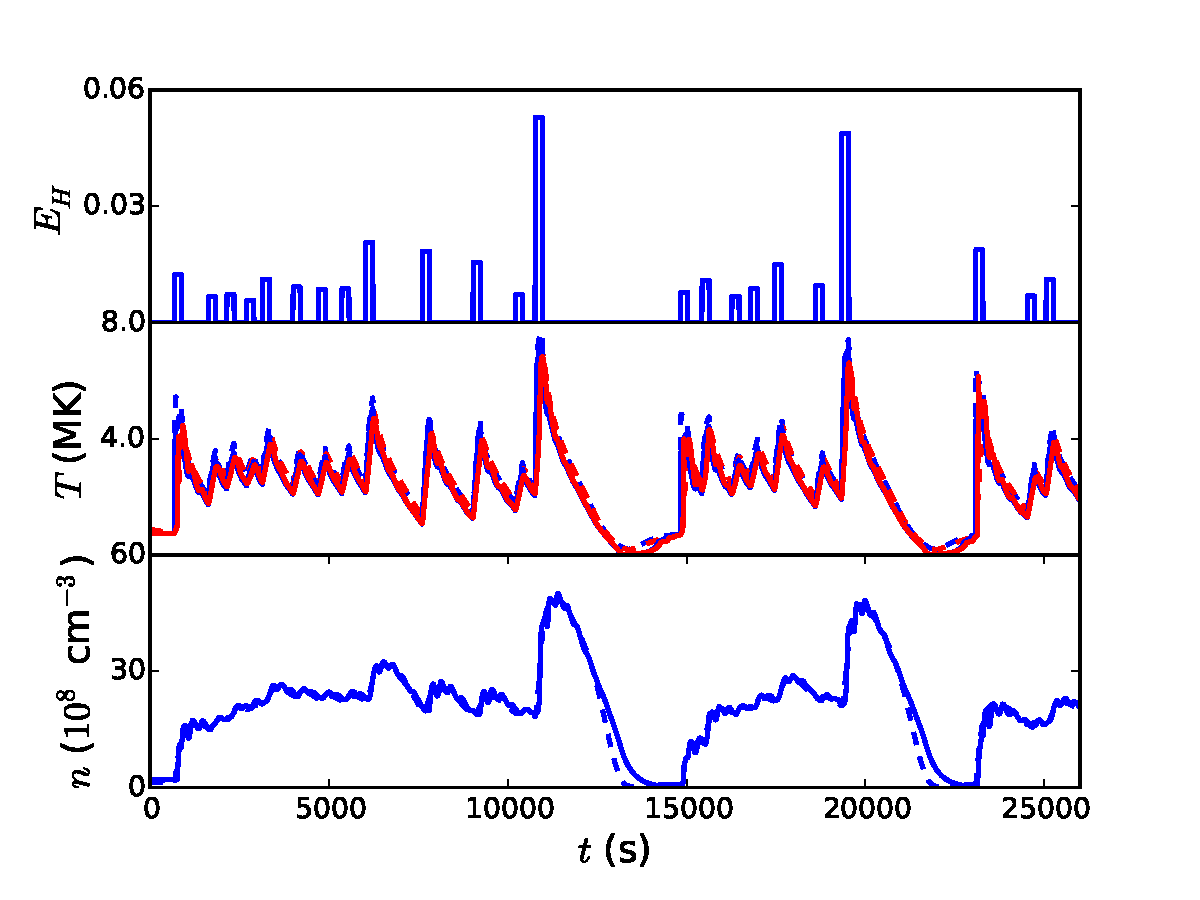
\includegraphics[width=\figwidth\columnwidth]{figures/compare_m_event.pdf}
					\label{fig:compare_m_event}}
					\caption{\ref{fig:compare_1_event} Comparison between two-fluid EBTEL model and HYDRAD for loop with half-length 25 Mm. EBTEL $T$ and $n$ profiles are apex quantities due to averaging in HYDRAD profiles. Heating is triangular pulse lasting 500 s with amplitude 0.05 erg cm$^{-3}$ s$^{-1}$. \ref{fig:compare_m_event} Same as Fig. \ref{fig:compare_1_event}, but for a series of 23 square pulses, each lasting 200 s with amplitudes chosen from a power-law distribution. $E_H$ is in units of $\mathrm{erg}~\mathrm{cm}^{-3}~\mathrm{s}^{-1}$.}
					\label{fig:hydrad_compare}
				\end{figure}
				\vspace{-2ex}
			\end{block}
			%Heating functions
			\begin{block}{Heating Function}
				\begin{itemize}
					\item Amplitudes either uniform or chosen from power-law distribution
					\item Power-law runs are constructed such that total number of events is representative of index $\alpha$ independent of heating frequency (see Fig. \ref{fig:heat_stats})
					\item Amplitudes are chosen such that for each run, time-averaged heating rate $H_n$ is sufficient to keep a loop in hydrostatic equilibrium at a temperature of $\sim4$ MK, consistent with observations \citep{warren_constraints_2011,warren_systematic_2012}.
					\item Heating applied to electron (ion) species through $E_H$ term in Eq. \ref{eq:ebtf_pe} (\ref{eq:ebtf_pi})
					\item Vary heating frequency such that $250\leq T_N\leq5000$ s in increments of $250$ s, where $T_N$ is the time between consecutive heating events (see Fig. \ref{fig:heat_funcs})
				\end{itemize}
				\begin{figure}[htp]
					\centering
					\subfigure[]{%
					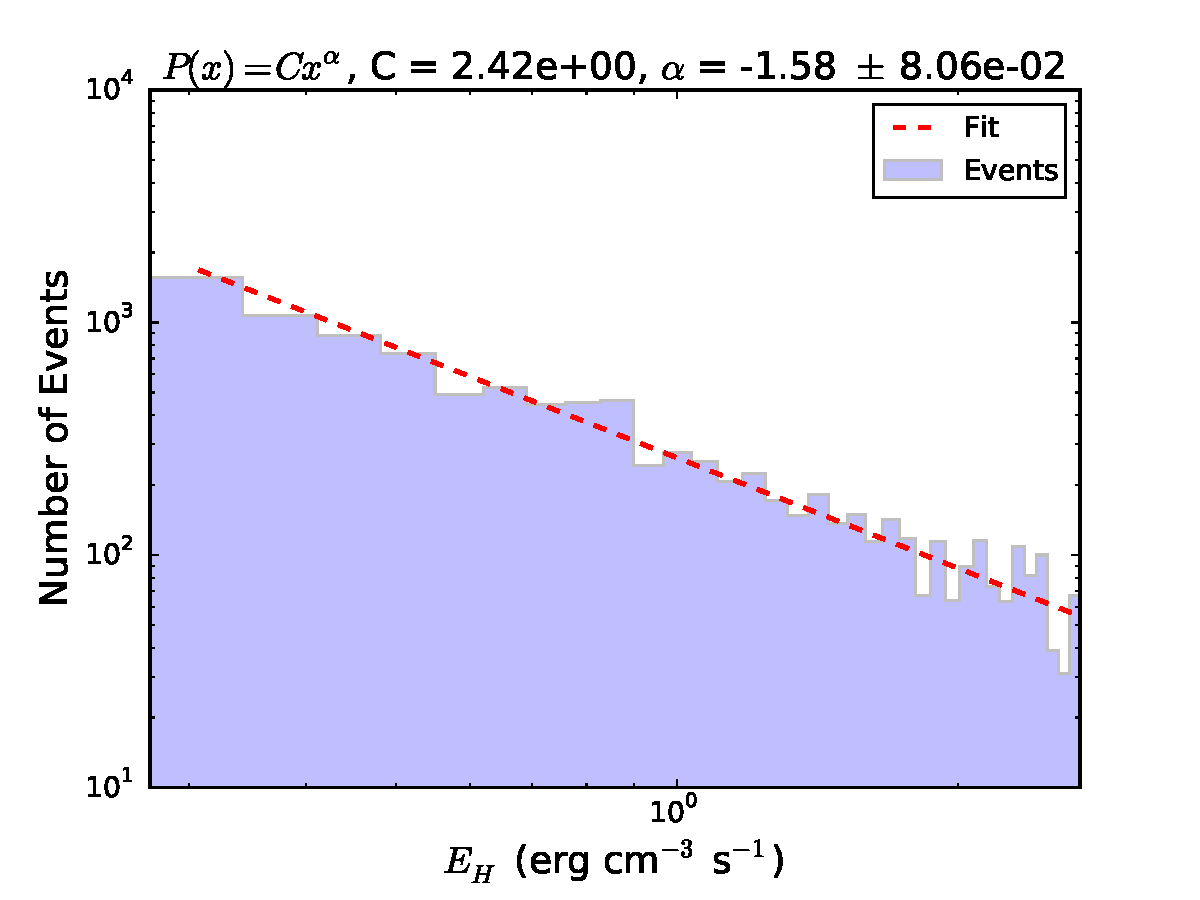
\includegraphics[width=\figwidth\columnwidth]{figures/heating_stats.pdf}
					\label{fig:heat_stats}}
					\subfigure[]{%
					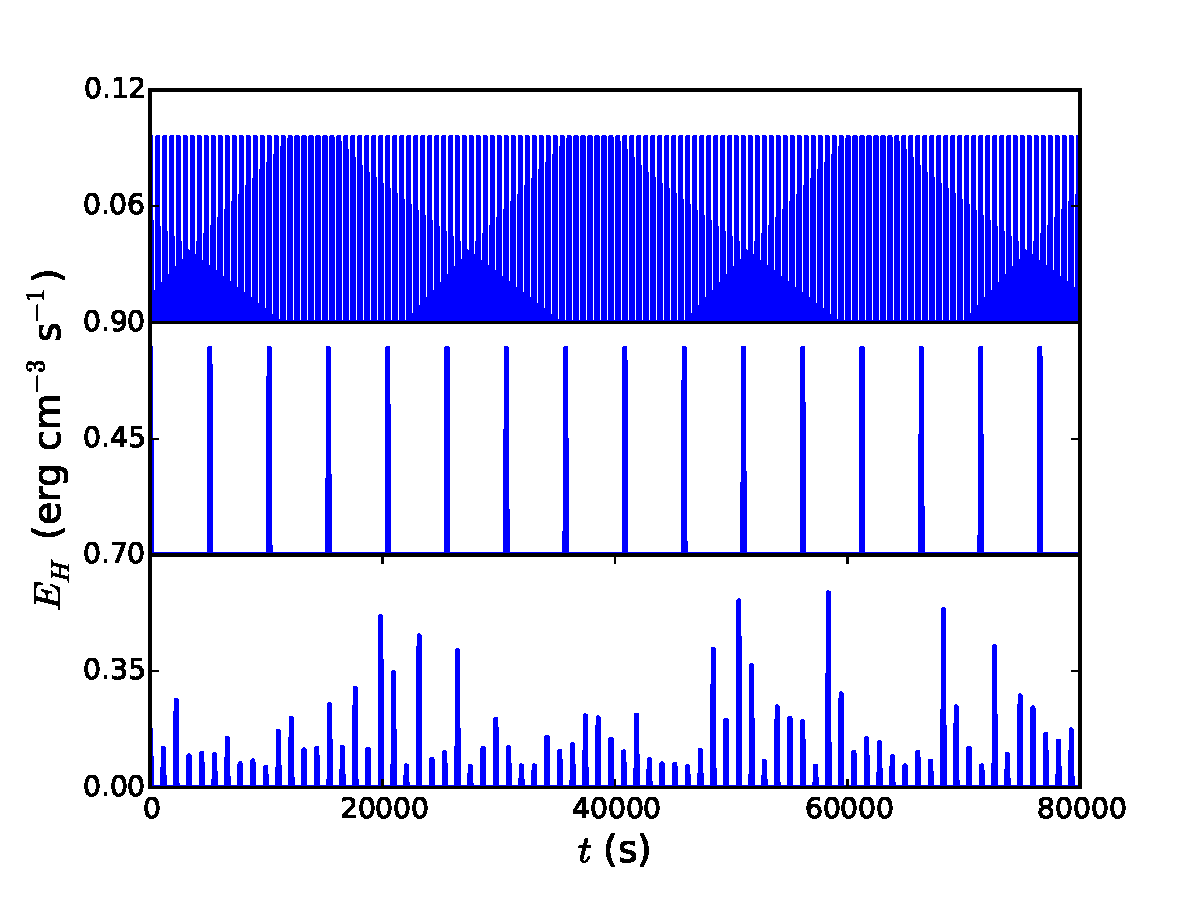
\includegraphics[width=\figwidth\columnwidth]{figures/heating_functions.pdf}
					\label{fig:heat_funcs}}
					\caption{\ref{fig:heat_stats} Resulting amplitude distribution for $\alpha=-1.5$, $L=40$ Mm, $T_N=5000$ s. For each $T_N$ value, $10^4$ events are included such that the power-law distribution is adequately represented. \ref{fig:heat_funcs} Sample heating functions for \textbf{top:} uniform amplitudes, $T_N=500$ s, \textbf{middle:} uniform amplitudes, $T_N=5000$ s, and \textbf{bottom:} power-law distributed amplitudes ($\alpha=-1.5$), $T_N=1000$ s. All events are 100 s in duration. In this study, we have used $250<T_N<5000$ s and $\alpha=-1.5,-2.0,-2.5$}
					\label{fig:heating}
				\end{figure}
				\vspace{-1ex}
			\end{block}
		\end{column}
		\begin{column}{0.49\linewidth}
			%Results
			\begin{block}{Emission Measure Curves}
				\vspace{-2ex}
				\begin{figure}[htp]
					\centering
					\subfigure[]{%
					\includegraphics[width=\figwidth\columnwidth]{figures/{ebtel_L40.0_tpulse100.0_alphauniform_electron_heating_dem}.pdf}
					\label{fig:em_uniform_electron}}
					\subfigure[]{%
					\includegraphics[width=\figwidth\columnwidth]{figures/{ebtel_L40.0_tpulse100.0_alpha1.5_electron_heating_dem}.pdf}
					\label{fig:em_a15_electron}}\\[-0.5ex]
					\subfigure[]{%
					\includegraphics[width=\figwidth\columnwidth]{figures/{ebtel_L40.0_tpulse100.0_alpha1.5_ion_heating_dem}.pdf}
					\label{fig:em_a15_ion}}
					\subfigure[]{%
					\includegraphics[width=\figwidth\columnwidth]{figures/{ebtel_L40.0_tpulse100.0_alpha1.5_single_heating_dem}.pdf}
					\label{fig:em_a15_single}}\\[-0.5ex]
					\caption{Emission measure curves constructed in the manner of \citet{cargill_active_2014} using $\mathrm{EM}=n^2L$ and method of \citet{klimchuk_highly_2008} for half-length of $L=40$ Mm using the Raymond-Klimchuk loss function with overlaid hot- and cool-branch fits for \ref{fig:em_uniform_electron} electron heating, $\alpha=$uniform, \ref{fig:em_a15_electron} electron heating, $\alpha=-1.5$, \ref{fig:em_a15_ion} ion heating, $\alpha=-1.5$, and \ref{fig:em_a15_single} both species heated equally (single-fluid EBTEL code) and $\alpha=-1.5$. \alert{Each curve is separated by an artificial spacing of 0.2 with different curves corresponding to differing values of $T_N$; bottom curve corresponds to $T_N=250$ s, the next curve $T_N=500$ s, and so on up to $T_N=5000$ s.}}
					\label{fig:em_curves}
				\end{figure}
				\vspace{-2ex}
			\end{block}
			\begin{block}{Emission Measure Slopes}
				\vspace{-2ex}
				\begin{figure}[htp]
					\centering
					\subfigure[]{%
					\includegraphics[width=\figwidth\columnwidth]{figures/{ebtel_L40.0_tpulse100.0_alphauniform_electron_heating_hs_compare}.pdf}
					\label{fig:slope_uniform_electron}}
					\subfigure[]{%
					\includegraphics[width=\figwidth\columnwidth]{figures/{ebtel_L40.0_tpulse100.0_alpha1.5_electron_heating_hs_compare}.pdf}
					\label{fig:slope_a15_electron}}\\[-0.5ex]
					\subfigure[]{%
					\includegraphics[width=\figwidth\columnwidth]{figures/{ebtel_L40.0_tpulse100.0_alpha1.5_ion_heating_hs_compare}.pdf}
					\label{fig:slope_a15_ion}}
					\subfigure[]{%
					\includegraphics[width=\figwidth\columnwidth]{figures/{ebtel_L40.0_tpulse100.0_alpha1.5_single_heating_hs_compare}.pdf}
					\label{fig:slope_a15_single}}\\[-0.5ex]
					\caption{Same as Fig. \ref{fig:em_curves}, but for emission measure slope values, $a$ in well-known scaling $\mathrm{EM}\propto T^a$, calculated from linear fits to hot (red) and cool (blue) branches for varying $T_N$. All cool branches are fit on the interval $6.0\leq\log(T)\leq6.6$ while the limits on the hot branches are $6.8\lesssim\log(T)\lesssim7.3$ and adjusted such that the fit is always done hotward of the temperature of peak $\mathrm{EM}$ with an upper limit placed at roughly where the $\mathrm{EM}$ curve begins to drop off sharply. Ion heating $\mathrm{EM}$ curves have no hot-shoulder fit because the $\mathrm{EM}$ value drops off sharply after the peak. Error bars correspond to $1\sigma$ calculated over many runs used to properly sample power-law distribution.}
					\label{fig:em_slopes}
				\end{figure}
				\vspace{-2ex}
			\end{block}
			\begin{block}{Conclusions}
				\vspace{-1ex}
				\begin{itemize}
					\item \alert{Pronounced hot shoulder for electron-only heating (uniform and $\alpha=-1.5$) while single-fluid case shows nearly linear hot branch, no visible hot shoulder}
					\item In electron-only heating, no energy partitioned to ions $\rightarrow$ more high-$T$ emission
					\item Ion-only heating shows sharp drop hotward of peak; $T_e$ never ``sees'' peak ion temperature because of collisional coupling timescale
					\item For all cases, \alert{$2\leq a_{\mathrm{cool}}\leq3$ for $T_N\geq3000$ s, consistent with $2\lesssim a_{\mathrm{cool}}\lesssim5$} reported in observations and simulations \citep[see Table 3 of][]{bradshaw_diagnosing_2012}
					\item $3\lesssim a_{\mathrm{hot}}\lesssim7$ though single-fluid case is only one well-described by linear fit (see Fig. \ref{fig:em_a15_single})
					\item Future work: \alert{improved calculations of $\mathrm{EM},~\mathrm{DEM}$ through forward modeling and $\mathrm{EM}$-loci or MCMC \citep{kashyap_markov-chain_1998} method}; more realistic determination of input-energy budget (i.e $Q\propto T_N,T_N^2$ \citep{cargill_active_2014})
				\end{itemize}
			\end{block}
			%References
	  	  	\begin{block}{References}
	  	  		\scriptsize
				\begin{multicols}{2}
	  			\bibliographystyle{apj}
	  	  		\bibliography{astrophys-abbrev.bib,references.bib}
				\end{multicols}
	  	  \end{block}
		\end{column}
	\end{columns}
\end{frame}
\end{document}
